\documentclass{article}

\usepackage{amsfonts}
\usepackage{amsmath}
\usepackage{xcolor}
\usepackage{textcomp}
\usepackage{graphicx}

\usepackage{listings}
\lstset{
	basicstyle=\ttfamily\color{olive}
}

\title{ECE-210-B HW3}
\author{Instructor: Jonathan Lam}
\date{Spring 2021}

\begin{document}
	\maketitle
	
	\noindent This homework reviews indexing and functions as covered in class.
	
	\begin{enumerate}
		\item
		Let's look at images! This question uses \lstinline|imshow| (see the help page!) and logical indexing to produce some simple shapes and show how we can use them as masks for image manipulation.
		
		\begin{enumerate}
			\item Create the logical matrix $A\in M_{256\times 256}(\mathbb{F}_2)$ where $a_{ij}$ is true iff $\sqrt{(i-128)^2-(j-128)^2}<64$. (Use \lstinline|meshgrid| or broadcasting.)
			
			($\mathbb{F}_2$, or Galois-field 2, is the field consisting of only the values $\{0,1\}$ and whose operations are akin to logical operators. For our purposes, these are the two logical values corresponding to false and true.)
			
			\item Create the logical matrix $B\in M_{256\times 256}(\mathbb{F}_2)$ where $b_{ij}$ is true iff $\sqrt{(i-96)^2-(j-96)^2}<64$.
			
			\item Create the following logical matrices. For each one, use \lstinline|figure| and \lstinline|imshow| to visualize it. Briefly describe each one in a comment.
			\begin{enumerate}
				\item $A$
				\item $B$
				\item $C=A\cap B^C$
				\item $D=A^C\cup B$
			\end{enumerate}
		
			\item Given the following matrices, and visualize them using \lstinline|figure| and \lstinline|imshow|. What do the \lstinline|.*| and \lstinline|+| operators do when dealing with logical arrays (``layer masks'')?
			\begin{lstlisting}
E = rand(256);
F = linspace(0, 0.25, 256) + linspace(0, 0.25, 256).';
G = E .* C + F .* D;
			\end{lstlisting}
			
			\item \textit{(Optional)} Rather than putting each plot in a new figure, use subplots using \lstinline|subplot| or \lstinline|tiledlayout|. Label each plot!
			
			\item \textit{(Optional)} Implement a function, \lstinline|generate_circle(x,y,rad)| that takes in the coordinates of the circle's center and its radius, and generates a $256\times 256$ logical matrix, and use it for parts (a) and (b). Alternatively, use it to generate arbitrary circles and visually demonstrate the inclusion-exclusion principle by \lstinline|xor|-ing all the circles.
		\end{enumerate}
	
		\clearpage
		\item
		Calculus time!
		\begin{enumerate}
			\item Write a function \lstinline|deriv(y, x)| and \lstinline|antideriv(y, x)| which take vectors \lstinline|y| and \lstinline|x|, and which perform numerical differentiation and integration on the function $y=y(x)$. These should each output vectors of the same length as the input; you may need to pad your result with an arbitrary value. You did this already; now make it a function.
			
			\item Write a function \lstinline|switchsign(x)| which takes a vector \lstinline|x| and returns a logical array with the same length as \lstinline|x| that is true when \lstinline|x| switches sign. E.g., for \lstinline|x=[2 3 -1 0 -1 5]| it would return \lstinline|[0 0 1 0 0 1]|. Do not use a \lstinline|for| loop.
			
			(Hint: One way to vectorize this is to use the \lstinline|sign| and \lstinline|diff| functions. Another way is to write conditions on the vector and use a shifted version of itself. You will probably need to pad the resulting vector to make it the same length as the original vector; one way to do this is to repeat the first element of the resulting vector twice.)
			
			\item Write a function \lstinline|extrema(y, x)| that uses the first derivative test to find local extrema (minima and maxima). Recall that local extrema on a differentiable function occur when $y'(x)$ changes sign. Use your \lstinline|deriv| and \lstinline|switchsign| functions here. The output of this function should also be two vectors: one representing the $y$ values of the extrema, and one representing the corresponding $x$ values.
			
			\item Write a function \lstinline|inflections(y, x)| that uses the second derivative test to find inflection points (i.e., when $y''(x)$ changes sign).
			
			\item Let $x$ be a 1001-point vector linearly spaced from $-2\pi$ to $2\pi$. Use \lstinline|sinc| to generate $y=\text{sinc}(x)$ over this interval. Generate the following variables using the functions you just wrote:
			\begin{enumerate}
				\item \lstinline|y_antideriv|, the antiderivative of $y$
				\item \lstinline|y_deriv|, the derivative of $y$
				\item \lstinline|y_extr| and \lstinline|x_extr|, the coordinates of the local extrema of $y$
				\item \lstinline|y_infl| and \lstinline|x_infl|, the coordinates of the inflection points of $y$
			\end{enumerate}
			Plot these using: \begin{lstlisting}
plot(x,y,x,y_antideriv,x,y_deriv, ...
     x_extr,y_extr,'r*',x_infl,y_infl,'bo');
			\end{lstlisting}
			Title your plot and label the axes. It should look something like:
			\begin{figure}[!h]
				\centering
				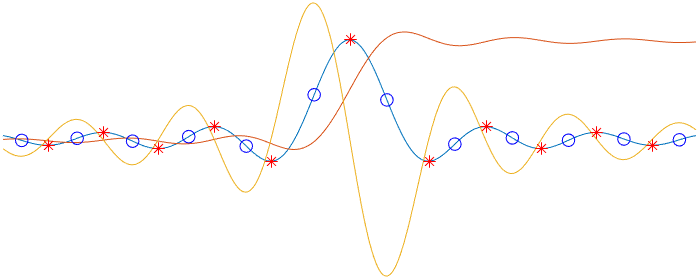
\includegraphics[width=2.5in]{result.png}
			\end{figure}
		\end{enumerate}
	\end{enumerate}
	
\end{document}